% This file was created with tikzplotlib v0.10.1.
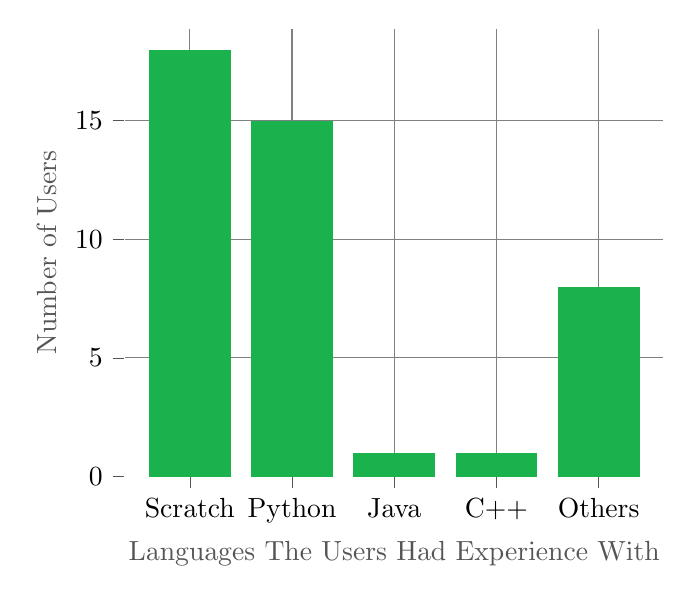
\begin{tikzpicture}

\definecolor{dimgray85}{RGB}{85,85,85}
\definecolor{gray}{RGB}{128,128,128}
\definecolor{limegreen2517876}{RGB}{25,178,76}

\begin{axis}[
axis line style={white},
tick align=outside,
tick pos=left,
x grid style={gray},
xlabel=\textcolor{dimgray85}{Languages The Users Had Experience With},
xmajorgrids,
xmin=-0.64, xmax=4.64,
xtick style={color=dimgray85},
xtick={0,1,2,3,4},
xticklabels={Scratch,Python,Java,C++,Others},
y grid style={gray},
ylabel=\textcolor{dimgray85}{Number of Users},
ymajorgrids,
ymin=0, ymax=18.9,
ytick style={color=dimgray85}
]
\draw[draw=none,fill=limegreen2517876,very thin] (axis cs:-0.4,0) rectangle (axis cs:0.4,18);
\draw[draw=none,fill=limegreen2517876,very thin] (axis cs:0.6,0) rectangle (axis cs:1.4,15);
\draw[draw=none,fill=limegreen2517876,very thin] (axis cs:1.6,0) rectangle (axis cs:2.4,1);
\draw[draw=none,fill=limegreen2517876,very thin] (axis cs:2.6,0) rectangle (axis cs:3.4,1);
\draw[draw=none,fill=limegreen2517876,very thin] (axis cs:3.6,0) rectangle (axis cs:4.4,8);
\end{axis}

\end{tikzpicture}
